
% !TEX root = TD_fluides_part1.tex



\section{Exercices de synthèse }


\setcounter{subsection}{-1}

%--------------------------------------------------------------------------------------------------
\subsection{Amortisseur hydraulique (partiel 2017; correction sur moodle)}
%--------------------------------------------------------------------------------------------------

On consid\`ere un amortisseur constitu\'e d'un piston de rayon $R=20$ mm et de longueur $L=20$ mm coulissant dans un cylindre de rayon $R+a$, avec $a =0.1$ mm. Ce cylindre est rempli d'une huile de viscosit\'e dynamique $\mu=0.1$Pa.s.\\
On veut d\'eterminer la relation entre la force $F$ appliqu\'ee sur le piston et sa vitesse $V$ par rapport au cylindre. Le fluide dans les deux chambres sup\'erieure et inf\'erieure au piston sera consid\'er\'e au repos. L'\'ecoulement,dans l'interstice (le jeu) entre les parois lat\'erales du piston et du cylindre, est visqueux (newtonien), stationnaire et \'etabli . Il sera approxim\'e \textit{localement} par l'\'ecoulement \'etabli entre deux plaques planes distantes de $a$, de longueur $L$, de largeur $2\pi R$ (p\'erim\`etre {\it d\'eroul\'e}). On consid\'erera que les pressions $p_i$ et $p_a$ dans les chambres inf\'erieure et sup\'erieure sont uniformes, et que la contribution hydrostatique, d'ordre $\rho gL$, est n\'egligeable devant $p_i-p_a$.\\


\begin{figure}[hbt]
  \begin{center}
    \setlength{\unitlength}{1mm}
    \begin{picture}(100, 60)(0, 0)
      \put(0, 0){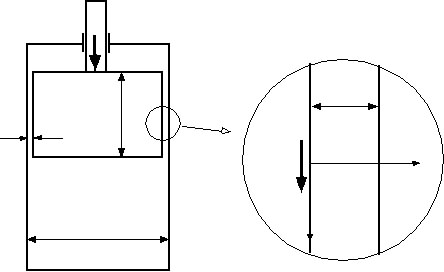
\includegraphics[width=10cm]{Figures/Amortisseur.jpg}}
      \put(1, 32){$a$}
      \put(20, 55){$F$}
      \put(23, 34){$L$}
      \put(15, 9){$2(R+a)$}
      \put(10, 48){$p_a$}
      \put(20, 20){$p_i$}
      \put(66, 10){$x$}
      \put(89, 27){$y$}
      \put(63, 25){$V$}
      \put(76, 39){$a$}
    \end{picture}
  \end{center}
  \label{fig:amortisseur}
  \caption{Sch\'ema de l'amortisseur hydraulique.}
\end{figure}

\begin{enumerate}

\item On suppose un écoulement parallèle stationnaire décrit en coordonnées cylindriques par $\vec u=u(r) \vec{e}_r$ et un champ de pression $p(x)$. 
A partir des équations de Navier-Stokes en coordonnées cylindriques (Formulaire, section D.2), Ecrire l'équation différentielle vérifiée par $u(r)$.


%  avec $y=r-R$ pour la vitesse axiale dans l’interstice entre le piston et le cylindre.  Expliquer succinctement pourquoi on peut négliger localement les effets de courbure sur le profil de vitesse et approximer $u$ par $u(y)$ (au lieu de $u(r,\theta,x)$ !)

%Estimez q

\rep{
$$
-\frac{\partial p}{\partial x} + \mu \left( \frac{\partial^2 u}{\partial r^2} 
+  \frac{1}{r}  \frac{\partial u}{\partial r} \right) = 0 ;%\quad \frac{\partial p}{\partial y}=0
$$
}
  
\item 
Par analyse des ordres de grandeurs des termes de l'équation, montrez que si $a\ll R_1$ le terme de courbure apparaissant dans la partie visqueuse peut être négligé, et qu'après le changement de variable $y = r-R_1$ l'équation se simplifie en :

$$
-\frac{\partial p}{\partial x} + \mu \frac{\partial^2 u}{\partial y^2} = 0 %\quad \frac{\partial p}{\partial y}=0
$$



\rep{
%Ayant justifié que le profil est de la forme $\myvec{u} = [u(y), 0, 0]$ , on injecte cette solution dans les équations de Navier-Stokes.  En ne gardant que les termes non nuls, on aboutit aux équations demandées.
L'ordre de grandeur du terme $\frac{\partial^2 u}{\partial r^2}$ et $[U]/a^2$ et celui du terme  $\frac{1}{r}  \frac{\partial u}{\partial r}$ est $[u]/(R_1 a)$, le rapport des deux est $a/R_1 \ll 1$, 
on peut donc négliger le second.
}


 Qu'en déduit-on sur la pression et son gradient suivant $x$ ?

\rep{ En dérivant la première équation selon $x$ on a  $\frac{\partial^2 p}{\partial x^2}=0$. La pression est une fonction linéaire de $x$ et son gradient est constant.
} 

\item 
Établir l'expression du profil de vitesse $u(y)$ et montrer qu'il correspond à la somme d'un écoulement de Poiseuille proportionnel à $-\partial p/\partial x$ et d'un écoulement de Couette proportionnel à $V$. 

\rep{
En intégrant deux fois selon $y$ et en tenant compte des conditions limites $u(0)= V$ et $u(a) = 0$, on trouve : 
$$ 
u(y) = V \cdot \left( 1 - \frac{y}{a} \right) + \frac{a^2}{2\mu} \frac{\partial p}{\partial x} \frac{y}{a} \left( 1 - \frac{y}{a} \right)   
$$
On reconnait un écoulement de Couette et un écoulement de Poiseuille.
}


\item Calculez le débit volumique à travers l'interstice. On distinguera la contribution $Q_p$  associée à l'écoulement de Poiseuille et la contribution $Q_c$ associée à l'écoulement de Couette.

\rep{
Ce débit (compté du bas vers le haut) vaut :
$$
Q = - \int_R^{R+a} u(r) 2 \pi r dr d \theta \approx - L \int_0^a u(y) dy = Q_c + Q_p
$$ 
$$ 
\mbox{ avec } Q_c = -\frac{V L a}{2} ; \quad Q_p = -\frac{a^2 L}{12 \mu}  \frac{\partial p}{\partial x}
$$
}

%\i

\item Montrer que le débit volumique chassé par le piston est égal à $Q = \pi R^2 V$.

\rep{Au cours d'un instant $dt$ le piston chasse un volume $d{\cal V} = \pi R^2 V dt$ vers le haut, 
le débit volumique est donc $Q = d{\cal V}/dt = \pi R^2 V$.}


\item En déduire que le gradient de pression est donné (à l'ordre dominant) par 
$(p_i-p_a)/L = 6 \mu R V/a^3$ .

On justifiera au passage que le débit associé à l'écoulement de Couette est négligeable devant celui associé à l'écoulement de Poiseuille.

\rep{ 
On écrit maintenant $Q = Q_p+ Q_v$, ce qui conduit à :
$$
\frac{\partial p}{\partial x} = \frac{6\mu R V}{a^3} \left( 1+\frac{a}{R} \right)  \approx  \frac{6\mu R V}{a^3}
$$
Le terme négligé $a/R$ correspond effectivement au rapport $Q_c/Q$.
}





\item  Montrez que la force exercée sur le piston se compose de trois termes, notés respectivement $F_P$ (résultante des efforts de pression), $F_{v,c}$ (résultante des contraintes visqueuses associées à l'écoulement de Couette), et $F_{v,p}$ (résultante des contraintes visqueuses associées à l'écoulement de Poiseuille).

Exprimez $F_p, F_{v,c}$ et $F_{v,p}$ en fonction des données du problème.

\rep{
$$
\myvec{F} = \int_S (-p \myvec{n} + \tau \cdot \myvec{n} ) dS   
$$
En projetant selon l'axe $x$ on a $F = F_p+F_{v,c}+F_{v,p}$ avec respectivement :
$$
F_p = 6 \pi \mu V \frac{R^3}{a^3} ; \quad 
F_{v,p} = 12 \pi \mu L V R^2/a^2 ; \quad 
F_{v,c} = 2 \pi \mu L V R/a.
$$
}

\item Comparez l'ordre de grandeur de ces trois forces, et montrez qu'à l'ordre dominant la force totale a pour expression $F = 6 \pi \mu V \frac{R^3}{a^3}$.

\rep{C'est la contribution $F_p$ qui domine.}

\item Application : Quelle force faut-il appliquer pour imprimer une vitesse de $1cm/s$ au piston ? L’écoulement est-il laminaire ? 

\rep{ $F =1.5\cdot 10^5 N$, force équivalant à 15 tonnes ! 
Le Reynolds est de l'ordre de la centaine, l'écoulement reste donc laminaire.}


%\item  Calculer les contraintes de cisaillement liées d’une part à l’écoulement de couette et d’autre part à l’écoulement de Poiseuille. Sont-elles du même ordre ? Laquelle a été négligée dans le calcul de la force F appliquée au piston ?

\end{enumerate}



\subsection{Ecoulement de Couette-Taylor}
%% Exo récupéré d'archives L2.

\begin{center}
\input{./Figures/CouetteTaylor.pstex_t}
\end{center}



On considère l'écoulement entre deux cylindres coaxiaux de rayon 
$R_1$ et $R_2$, et de hauteur $H$.
Le cylindre intérieur tourne à la vitesse angulaire $\Omega$ autour
de son axe $e_z$, et le cylindre extérieur est fixe. 
Le fluide remplissant l'espace entre les deux cylindres est 
newtonien et incompressible, 
de masse volumique $\rho$, viscosité dynamique $\mu$ 
(et viscosité cinématique $\nu=\mu/\rho$). On néglige l'effet de la gravité.

L'écoulement est azimutal, c'est à dire de la forme 
$\vec u = v(r) \vec e_\theta$. 


%Question préliminaire : que vaut $\tau_{\theta r}$ pour un écoulement
%de rotation pure, de la forme $v(r) = A r$ ? Expliquez physiquement.

{\bf A. Ecoulement stationnaire}


\begin{enumerate}


\item Rappelez l'expression de la composante $\tau_{\theta r}$ du tenseur des contraintes visqueuses (cf. formulaire, section D.2).

\rep{
$$
\tau_{\theta r} = \mu r \partial( v/r) /\partial r.
$$
}

\item On considère un volume de contrôle élémentaire 
$\delta V = d z \times d r \times (r d \theta)$. 
Calculez son moment cinétique $\delta \vec L_0$  par rapport à un point
 $O$ situé sur l'axe des cylindres.
 

\item En appliquant le théorème du moment dynamique au volume élémentaire
$\delta V$ et en projetant dans la direction $\vec e_z$, montrez que 
l'écoulement est gouverné par l'équation suivante (2), 
analogue pour un écoulement cylindrique azimutal de l'équation de Navier :

\begin{equation}
\rho \frac{\partial v}{\partial t} = - \frac{1}{r}\frac{\partial p}{\partial \theta}
+ \frac{\mu}{r^2}\frac{\partial}{\partial r}
\left[ r^3 \frac{\partial}{\partial r} \left( \frac{v}{r} \right) \right].
\end{equation}

\item Retrouvez cette équation a partir des équations de Navier-Stokes 
en coordonnées cylindriques (Formulaire, section D.2).

\item Justifiez pourquoi le gradient de pression $\partial p/\partial \theta$
est nul.

\item On cherche une solution stationnaire de l'équation (2).
Montrez que la solution générale est de la forme $v(r) = A r + B/r$.

\item Précisez les conditions aux limites $v(R_1)$ et $v(R_2)$.

\item En déduire la valeur des constantes $A$ et $B$.

\rep{
$A = ...$
$B = ...$
}

\item Calculez le moment global $\vec {\cal M}_O$ 
(par rapport au point $O$ de l'axe des
cylindres) des efforts exercés par le fluide sur
le cylindre intérieur, et montrez que
$$ 
\vec {\cal M}_O = - 4 \pi \mu H \Omega \frac{R_2^2 R_1^2}{R_2^2 -R_1^2} 
\vec e_z.
$$

\item Calculez le moment des efforts exercés par le fluide sur le cylindre intérieur. Que constatez-vous ?

\item Application : les dimensions du viscosimètre sont $R_1 = 20cm$, $R_2 =
21cm$, $H = 20cm$. On fait tourner le cylindre intérieur à la vitesse
$\Omega = 100 tours/s$, et on mesure un moment $|\vec {\cal M}_O| = 6 Nm$.
Donnez la viscosité dynamique du fluide. 

{\bf A. Ecoulement instationnaire}

Dans cette partie on pose $d = (R_2-R_1)$ et on suppose $d \ll R_1$.

On suppose que le taux de rotation du cylindre intérieur oscille de manière périodique avec une fréquence $f = 2 \pi \omega$ et une amplitude maximale $C$, c'est-à-dire :

$$
\Omega_1(t) = C  \cos (\omega t)
$$

Le cylindre extérieur est toujours supposé fixe ($ \Omega_2(t) = 0)$.

\item Montrez par analyse dimensionnelle que les termes de courbure peuvent être négligés et que l'équation se ramène à :

\begin{equation}
\frac{\partial v}{\partial t} = \nu \frac{\partial^2 v}{\partial s^2}
\end{equation}
 
 avec $s = (r-R_1)$.
 
 \item 
 Précisez les conditions limites vérifiées par $v(s,t)$ en $s=0$ et $s=d$.

 
\item On cherche la solution sous la forme 
$v(r,t) = Re ( \underline{v}(r) e^{-i \omega t} )$. 
Donnez l'expression de  $\underline{v}(r)$.

\item En posant $St = d^2 \omega/\nu$, que devient l'expression précédente dans la limite $St \ll 1$ ? Expliquez physiquement.

\item Que devient l'expression précédente dans la limite $St \gg 1$ ? Expliquez physiquement.


\end{enumerate}


%--------------------------------------------------------------------------------------------------
\subsection{Drainage entre deux disques rapproch\'es (d'apr\`es examen 2004) \exonormal}
%--------------------------------------------------------------------------------------------------

Deux disques circulaires plans de rayon $R=5$ cm sont dispos\'es parall\`element 
(fig.~\ref{fig:disques}) l'un au-dessus de l'autre. 
Dans l'espace entre les disques se trouve une huile de viscosit\'e dynamique $\mu = 6.26$ Pa s 
et de masse volumique $\rho = 1230$ kg/m$^3$. 
On consid\`ere que l'\'epaisseur de fluide $h$ entre les deux disques reste tr\`es petite 
devant le rayon $R$ : $h \ll R$. L'\'epaisseur $h_0$ \`a l'instant initial ($t=0$) est \'egale 
\`a $h_0=0,5$ cm. La pression \`a l'ext\'erieur des disques correspond \`a la pression 
atmosph\'erique $P_a$.

On exerce une force $\textbf{F} = F \textbf{e}_z$ sur le disque sup\'erieur afin de 
chasser lat\'eralement le fluide. Cette force impose au disque sup\'erieur une vitesse 
$\textbf{U} = U \textbf{e}_z$, le disque inf\'erieur restant fixe.

Dans un premier temps, on se propose de d\'eterminer l'intensit\'e $F(t)$ de la force qu'il faut 
exercer pour maintenir \emph{constante} la vitesse $U = 0,5$ mm/s du disque sup\'erieur. 
On s'attachera ensuite \`a d\'ecrire en d\'etail l'\'ecoulement entre les deux disques.

La couche de fluide \'etant mince et le probl\`eme axisym\'etrique, on consid\`ere que 
la pression ne d\'epend ni de $z$ ni de l'angle azimutal $\theta$, soit $p = p(r, t)$, 
et on cherche un champ de vitesse s'\'ecrivant : 
$\textbf{u} = u_r(r, z, t) \textbf{e}_r + u_z(r, z, t) \textbf{e}_z$.

\begin{figure}[hbt]
    \setlength{\unitlength}{1mm}
  \begin{center}
    \begin{tabular}{cc}
      \begin{picture}(75, 60)
	\put(0, 0){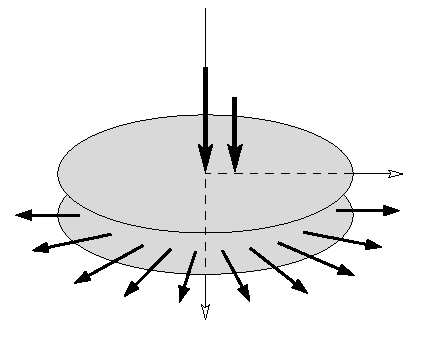
\includegraphics{disques1}}
	\put(60, 40){$P_a$}
	\put(31, 3){$z$}
	\put(65, 32){$r$}
	\put(30, 45){$\textbf{F}$}
	\put(42, 40){$\textbf{U}$}
      \end{picture}
      &
      \begin{picture}(75, 60)
	\put(0, 0){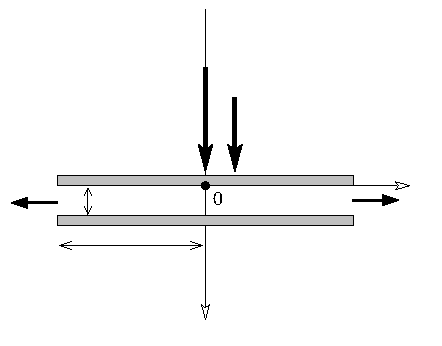
\includegraphics{disques2}}
	\put(20, 13){$R$}
	\put(65, 30){$r$}
	\put(30, 5){$z$}
	\put(17, 23.5){$h(t)$}
	\put(10, 35){$P_a$}
	\put(30, 45){$\textbf{F}$}
	\put(42, 40){$\textbf{U}$}
      \end{picture}
    \end{tabular}
  \end{center}
  \mycaption{Ecoulement visqueux entre deux disques.}
  \label{fig:disques}
\end{figure}

Les relations ci-dessous donnent, en coordonn\'ees cylindriques
$(r, \theta, z)$, la composante radiale de l'\'equation du mouvement
(\ref{eq:mvt}) et l'\'equation d'incompressibilit\'e (\ref{eq:cont}) : 
\begin{eqnarray}
\rho \left [  \dpa{u_r}{t} + u_r \dpa{u_r}{r} + u_z \dpa{u_r}{z} \right ]
&=& - \dpa{p}{r} + \mu \left[ 
\dpa{}{r} \left( \frac{1}{r}\dpa{}{r}(r u_r) \right) + \ddpa{u_r}{z} \right],
\label{eq:mvt} \\
\frac{1}{r} \dpa{}{r}(r u_r) + \dpa{u_z}{z} & = & 0.
\label{eq:cont}
\end{eqnarray} 

\begin{enumerate}
\item
  \begin{enumerate}
  \item 
    En choisissant $U$, $R$  et $[T] = R/U$ respectivement comme \'echelles caract\'eristiques
    de vitesse, de longueur et de temps, calculer la valeur du nombre de Reynolds et du nombre de Stokes pour cet \'ecoulement. Commenter.
  \item 
    Montrer que l'\'equation du mouvement peut se simplifier sous la forme :
    \begin{equation}
      \dpa{p}{r} = \mu \left[ \dpa{}{r} \left( \frac{1}{r}\dpa{}{r}(r u_r) \right) +
	\ddpa{u_r}{z} \right].
      \label{eq:smpl}
    \end{equation}
  \item 
    On cherche \`a simplifier davantage l'\'equation ci-dessus.
    En choisissant comme \'echelles de longueur $h$ suivant $z$, et $R$
    suivant $r$, pour estimer l'ordre de grandeur des d\'eriv\'ees partielles, 
    et sur la base de l'hypoth\`ese simplificatrice $h \ll R$, simplifier le terme de droite 
    de l'\'equation (\ref{eq:smpl}). A l'aide des conditions aux limites (adh\'erence aux parois), 
    en d\'eduire l'expression de la vitesse radiale $u_r$ en fonction du gradient radial 
    de pression:      
  \begin{equation}
    u_r(r, z, t) = \frac{1}{2\mu} z [z-h(t)] \dpa{p}{r}.
  \end{equation}
      \end{enumerate}
\item 
  \begin{enumerate}
  \item 
    En injectant cette expression dans l'\'equation d'incompressibilit\'e
    (\ref{eq:cont}), d\'eterminer $u_z(r, z, t)$ en fonction de $\mu$, $h$,
    $\partial p/\partial r$ et $\partial^2 p/\partial r^2$.
  \item 
    A l'aide des conditions aux limites sur $u_z$ en $z=0$ et $z = h(t)$, 
    en d\'eduire l'\'equation diff\'erentielle que doit v\'erifier $p$.
  \item 
    Montrer alors que la pression au sein du fluide a pour expression :
    \begin{equation}
      p(r, t) = P_a + \frac{3\mu U}{h(t)^3} (R^2 - r^2).
      \label{pression}
    \end{equation}
  \end{enumerate}
\item
  \begin{enumerate}
  \item 
    D\'eterminer le module $F$ de la force pressante n\'ecessaire pour maintenir
    la vitesse $U$.
  \item 
    Donner l'expression de $h(t)$ en fonction de $U$ et $h_0$.
  \item 
    Tracer et commenter la courbe $F(t)$.
  \item 
    Sachant que le disque sup\'erieur sch\'ematise le piston d'un v\'erin qui admet
    pour pression maximale $P_m = 10^7$ Pa, d\'eterminer l'\'epaisseur minimale
    $h_m$ de fluide que l'on ne peut \'eliminer en maintenant la vitesse $U$, et le temps 
    $t_m$ n\'ecessaire pour effectuer cette vidange partielle de l'interdisque. 
    Faire l'application num\'erique.
  \end{enumerate}
\item
  \begin{enumerate}
  \item 
    Connaissant dor\'enavant le champ de pression (\ref{pression}) dans l'\'ecoulement, 
    d\'eterminer compl\`etement la vitesse radiale $u_r$ en tout point
    ($r$, $z$) de l'interdisque.
  \item
    Tracer la courbe donnant le profil de vitesse $u_r$ en fonction de la variable
    sans dimension $z/h$ pour diff\'erentes valeurs du temps $t$
    ($0 \leq t \leq t_m$).
  \item
    Etablir l'expression de la composante axiale de la vitesse, $u_z(r, z, t)$.
  \item
    D\'eterminer la tangente de l'angle ($\beta$) que fait le vecteur vitesse
    du fluide avec le plan  horizontal.
    En d\'eduire sch\'ematiquement l'allure des lignes de courant dans
    l'interdisque.
  \end{enumerate}
\item
  \begin{enumerate}
  \item 
    D\'eterminer le d\'ebit volumique de fluide s'\'ecoulant \textit{radialement}
    vers l'ext\'erieur des deux disques. Discuter le r\'esultat obtenu.
  \item 
    D\'eterminer le d\'ebit volumique de fluide s'\'ecoulant \`a travers une
    section normale \`a l'axe des disques (autrement dit, \textit{horizontale}).
    Tracer ce d\'ebit en fonction de $z/h$ et commenter.
  \end{enumerate}
\end{enumerate}

\Archives{
\subsection{Pompage d'un liquide par entrainement}
\begin{center}
\input{./Figures/Pompage.pstex_t}
\end{center}

La figure ci-dessus représente un dispositif utilisés dans certains
procédés industriels pour faire monter un liquide d'un réservoir à un
autre situé plus haut. Le fluide monte à travers un canal 
parallèle, de largeur $a$ et de profondeur $b$, situé entre un tapis
roulant se déplacant à la vitesse $V_0$ et une paroi fixe.


On suppose que l'écoulement peut être considéré comme parallèle et établi 
dans tout le canal, c'est à dire que $\vec u(x,y,t) = u(y) \vec e_x$
pour tout $x \in [0,L]$. 

On suppose le fluide newtonien et incompressible, de masse volumique 
$\rho$ et de viscosité dynamique $\mu$. 

\begin{enumerate}

\item Donnez l'équation différentielle vérifiée par la vitesse 
$u(y)$ à l'intérieur du canal, et précisez les conditions aux 
limites $u(0)$ et $u(a)$.

\item Justifier pourquoi on peut considérer que le gradient de pression
$\partial p/\partial x$ est nul à l'intérieur du canal.

\item Déterminez le profil de vitesse $u(y)$. On l'exprimera en fonction
de $y/a$, et en faisant apparaître le paramètre adimensionnel 
$N = g a^2/(2 \nu V_0)$.

\item Calculez le débit volumique $Q_v$ du fluide dans le canal, 
et trouvez une condition sur $N$ pour que le système joue 
le rôle de pompe.

\item Donnez l'expression de la contrainte visqueuse $\tau_{xy}(y)$. 
En déduire la force $\vec F$ exercée sur le tapis roulant, puis
la puissance ${\cal P}_m$ fournie par le moteur.

\item Appliquez le théorème de l'énergie mécanique au fluide traversant 
le dispositif entre deux instants $t$ et $t+dt$. En déduire que la
puissance utile du dispositif vaut  ${\cal P}_u = Q_v \rho g H$ .

\item Calculez le rendement $\eta = {\cal P}_u / {\cal P}_m$ du dispositif.
Pour quelle valeur de $N$ ce rendement est-il maximal ?       
 
\end{enumerate}
}
\subsection{Aspiration d'une couche limite}

\begin{center}
\input{./Figures/CL_Aspi.pstex_t}
\end{center}


Dans les écoulements à grands nombres de Reynolds caractéristiques
de l'aérodynamique, l'écoulement autour d'obstacles est caractérisé
par la présence de couches limites. Dans certains cas ces couches limites
peuvent être affectées par un phénomène de décollement qui perturbe
grandement les écoulements. Une facon d'éviter ces effets consiste à 
aspirer la couche limite à travers une paroi poreuse.

Dans cet exercice on considère une plaque plane disposée parallèlement
à l'écoulement. Loin de la plaque (en $y \rightarrow \infty$), 
la composante axiale de vitesse vaut $U_0$, et la pression est uniforme
avec la valeur $p=p_a$.
A la paroi de la plaque, la vitesse vaut $\vec u = -v_a \vec e_y$, 
(avec $v_a >0$). 


\begin{enumerate}

\item Ecrire les équations de Navier-Stokes et de continuité 
dans le cas général d'un écoulement bidimensionnel
(de la forme $\vec u = u(x,y,t) \vec e_x+v(x,y,t) \vec e_x$)
et incompressible, en négligeant la gravité.

\item Simplifiez les équations précédentes pour le cas particulier d'un
écoulement stationnaire et invariant dans la direction axiale, 
c'est à dire de la forme $\vec u = u(y) \vec e_x + v(y) \vec e_y$. 

%\item Précisez les conditions limites particulières à ce problème, 
%en $y=0$ et en $y \rightarrow \infty$.

\item 
Montrez que $v(y)$ et la pression $p(x,y)$ sont uniformes.

\item 
Montrez que la vitesse axiale est solution de l'équation différentielle :
$$
%\frac{\partial u}{\partial t } - 
v_a \frac{\partial u}{\partial y } + \nu 
\frac{\partial^2 u}{\partial y^2 } = 0
$$
Avec des conditions limites en $y=0$ et $y \rightarrow + \infty$ que vous préciserez.


\item Donnez la solution $u(y)$ du profil de vitesse.

\item Calculez l'épaisseur de la couche limite $\delta$, définie comme
la position à laquelle $u(y = \delta ) = 0.99 u(y \rightarrow \infty)$.

\item Calculez la contrainte pariétale $\tau_{xy}(y=0)$. En déduire
la force exercée sur une plaque plane (supposée de longueur $L$ et de largeur
$b$.)

\item Faites les applications numériques pour les deux questions précédentes, avec les données $U_0 = 10 m/s$, $v_a= 0.1 m/$, $L = b = 1m$, le fluide étant de l'air à pression et température ambiante.

\end{enumerate}



\Archives{
%--------------------------------------------------------------------------------------------------
\subsection{Coulée de lave}
%--------------------------------------------------------------------------------------------------

\noindent
On considère une coulée de lave le long d'une pente d'angle $\alpha$ par rapport à l'horizontale
(fig.~\ref{fig:Huppert}a).
Cet écoulement de lave est de faible épaisseur par rapport à sa longueur, et prend la forme d'un film mince
dont la surface libre est donnée par $y=h(x, t)$, où $y$ est la direction perpendiculaire à la pente de direction $x$.
Sous l'effet de la pesanteur, la coulée s'étale en s'écoulant, entre les points d'abscisses $x=0$ et $x=X(t)$,
ce dernier correspondant au front de la coulée.
L'objectif est ici de déterminer la loi de propagation du front de la coulée.

\begin{figure}[htb]
  \begin{center}
    \setlength{\unitlength}{1mm}
    \begin{picture}(160, 35)(0, -2)
      \put(0, 0){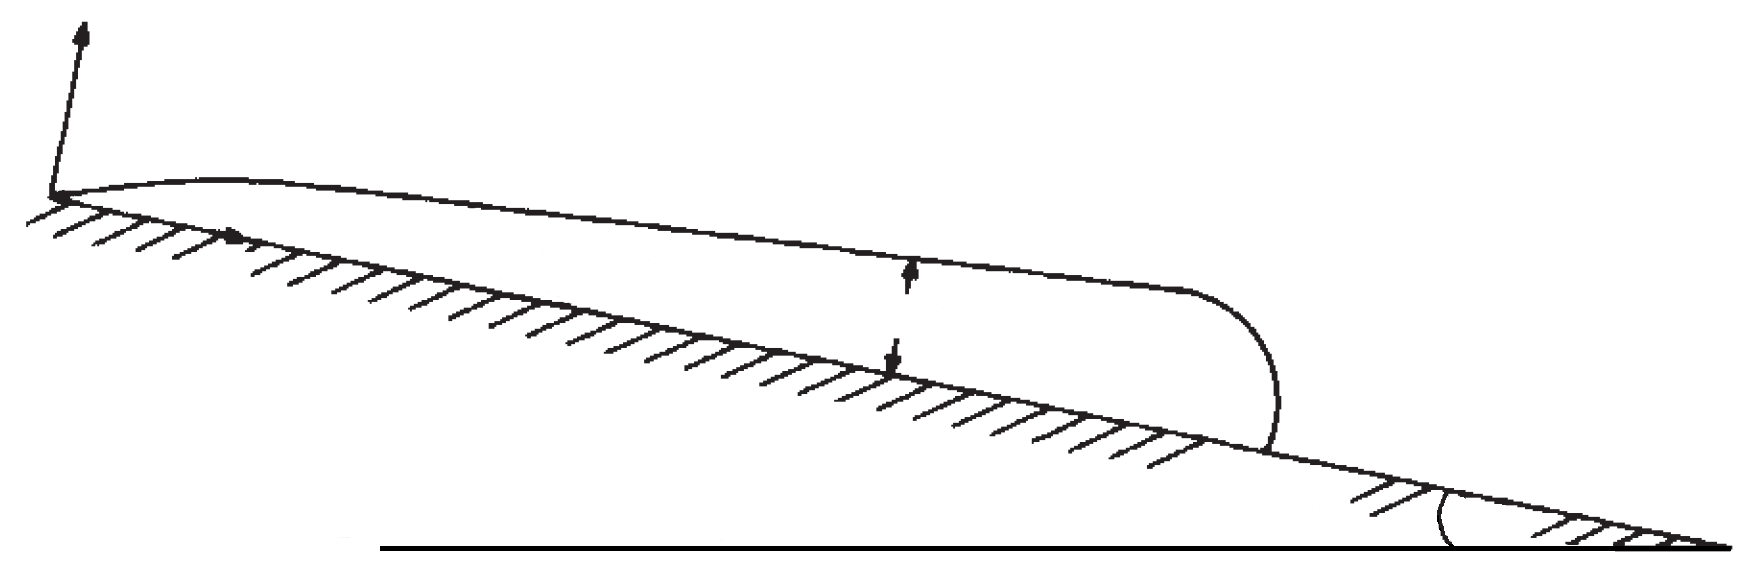
\includegraphics[width=9cm]{Huppert_geometry_clean.png}}
      \put(45, -6){(a)}
      \put(10.5, 15){\footnotesize $x$}
      \put(1, 27){\footnotesize	$y$}
      \put(0.5, 19){\footnotesize	$0$}
      \put(41.5, 13){\footnotesize $h(x, t)$}
      \put(60, 3.5){\footnotesize $X(t)$}
      \put(74.5, 2.4){\footnotesize $\alpha$}
      \put(70, 25){\thicklines \vector(0, -1){10}}
      \put(20, 22){\footnotesize $P_a$}
      \put(72, 20){\footnotesize $\myvec{g}=-g\,\myvec{e}_z$}
      \put(95, 1){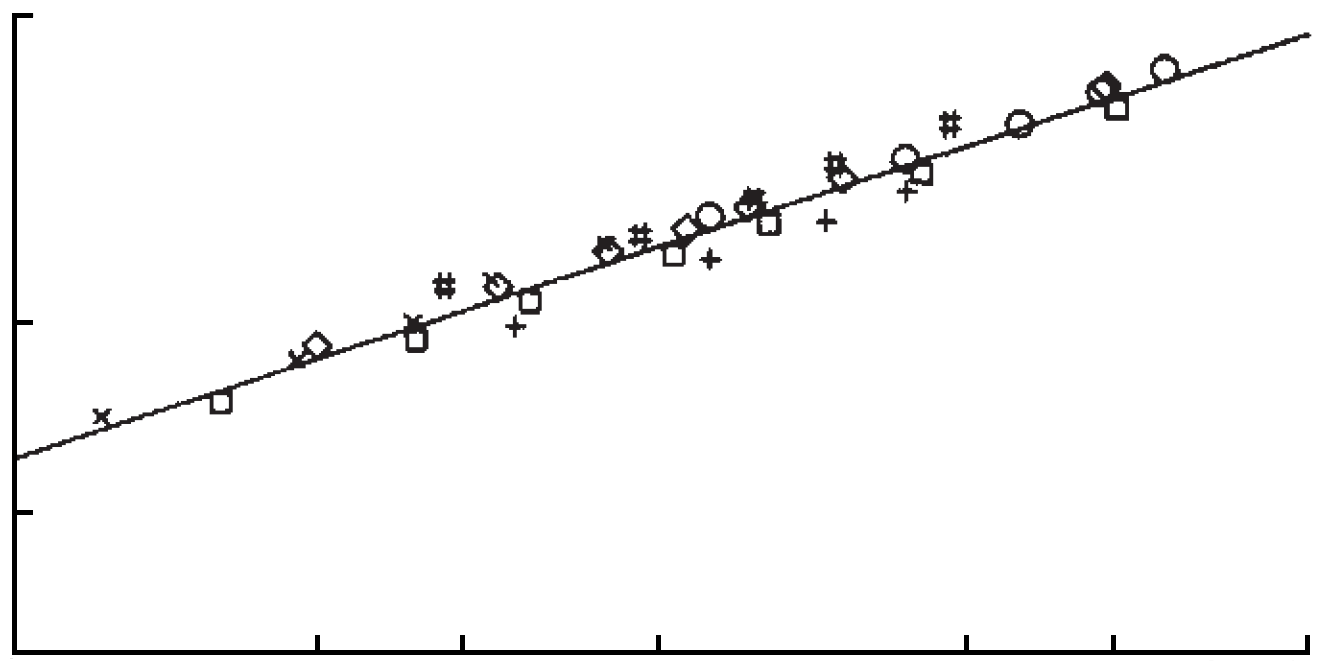
\includegraphics[width=6.5cm]{Huppert_results_clean.png}}
      \put(125, -6){(b)}
			\put(97, 30){\scriptsize $X(t)/\sqrt{S}$}
			\put(140, 4){\scriptsize $(g\sqrt{S}\sin\alpha/\nu)\, t$}
			\put(93, 0.7){\scriptsize $3$}
			\put(93, 7.7){\scriptsize $5$}
			\put(91.5, 16.9){\scriptsize $10$}
			\put(91.5, 31.9){\scriptsize $30$}
			\put(94, -2){\scriptsize $10^2$}
			\put(107, -2){\scriptsize $3.10^2$}
			\put(115, -2){\scriptsize $5.10^2$}
			\put(125, -2){\scriptsize $10^3$}
			\put(139, -2){\scriptsize $3.10^3$}
			\put(147, -2){\scriptsize $5.10^3$}
			\put(157, -2){\scriptsize $10^4$}
    \end{picture}
  \end{center}
  \mycaption{(a) : schéma de la coulée de lave. (b) : comparaison entre expérience (symboles) et prédiction théorique 
  	(droite de pente $1/3$ en échelle logarithmique). D'après Huppert (\textit{Nature} \textbf{300}, 427--429, 1982). }
  \label{fig:Huppert}
\end{figure}

\noindent
On supposera en première approximation que la lave est constituée d'un fluide homogène, 
de masse volumique $\rho$ uniforme, et newtonien, de viscosité cinématique $\nu$.
Dans l'hypothèse d'un écoulement incompressible, il est possible d'utiliser dans cette
configuration les équations de film mince pour la vitesse 
$\myvec{u} = u(x, y, t) \, \myvec{e}_x + v(x, y, t) \, \myvec{e}_y$
et la pression motrice $\hat{p} = p - \rho \, \myvec{g}\cdot \myvec{x}$ au point $\myvec{x}$ de coordonnées $(x, y)$~:
\[
	(1)\quad \frac{\partial^2 u}{\partial y^2} = \frac{1}{\mu} \, \frac{\partial \hat{p}}{\partial x},
	\qquad 
	(2)\quad \frac{\partial \hat{p}}{\partial y} = 0,
	\qquad
	(3)\quad \frac{\partial u}{\partial x} + \frac{\partial v}{\partial y} = 0,
	\quad \mbox{où $\mu = \rho \nu$ désigne la viscosité dynamique.}
\]
\begin{enumerate}
\item
	Montrer que la pression motrice s'écrit $\hat{p} = p(x, y, t) + \rho g (y\cos\alpha - x\sin\alpha)$.
\item
	En écrivant la continuité de la pression à l'interface $y=h(x, t)$, déduire de l'équation (2) 	
	que la pression au sein de la coulée a pour expression $p(x, y, t) = P_a + \rho g \cos\alpha\left [h(x, t)-y\right ]$ 
	où $P_a$ désigne la pression atmosphérique.
	En déduire la pression motrice $\hat{p}$.
\item
	Dans l'hypothèse de film mince, on peut supposer que $|\partial h/\partial x| \ll \tan\alpha$ pour $\alpha>0$.
	Montrer alors que $\partial \hat{p} / \partial x = -\rho g \sin\alpha$ en première approximation.
\item
	Dans ces conditions, résoudre l'équation (1) et montrer que $u(x, y, t) = -g\sin\alpha\; y^2/2\nu + A y + B$ où $A$ et $B$ sont
	deux fonctions de $x$ et $t$ à déterminer d'après les conditions aux limites en $y=0$ et $y=h(x, t)$.
	On négligera les frottements de l'air sur la coulée de lave.
\item
	Calculer le débit volumique le long de la coulée de lave : $q(x, t) = \displaystyle \int_0^{h(x, t)} u(x, y, t)\, dy$.
\item
	Montrer que la conservation de la masse implique que $\displaystyle \frac{\partial h}{\partial t} = -\frac{\partial q}{\partial x}$.
	On pourra admettre ce résultat.
\item
	Déduire des questions précédentes que $h(x, t)$ vérifie l'équation : 
	$\displaystyle \frac{\partial h}{\partial t} + \frac{g\sin\alpha}{\nu} h^2 \frac{\partial h}{\partial x} =0$.
\item
	Aux temps longs, on peut rechercher une solution, dite \textit{autosimilaire}, de la forme $h(x, t) = h_0\sqrt{x/t}$
	où $h_0$ est à déterminer en injectant ce type de solution dans l'équation pour $h$.
\item
		Le volume de cette coulée de lave étant fixé, $\displaystyle S = \int_0^{X(t)} h(x, t) \, dx$ est une constante du problème.
\item[]
		En déduire que la loi de propagation du front de lave s'écrit $X(t) = \sqrt{S} \; (t/\tau)^{1/3}$ 
		où $\tau$ est un temps caractéristique à déterminer en fonction des paramètres du problème (cf. fig.~\ref{fig:Huppert}b).	
\end{enumerate}

\hfill \textsl{(d'apr\`es partiel 2011)}
}

\Archives{
%--------------------------------------------------------------------------------------------------
\subsection{Ecoulement d'un film liquide d'\'epaisseur uniforme \exonormal}
%--------------------------------------------------------------------------------------------------

On consid\`ere un film liquide d'\'epaisseur uniforme s'\'ecoulant sur un plan inclin\'e 
d'un angle $\theta$ par rapport \`a l'horizontale. 
Soit $q$ le d\'ebit-volume impos\'e par unit\'e de largeur. 

\begin{enumerate}
\item 
  D\'eterminer le profil des vitesses $u(y)$ en fonction de l'\'epaisseur $h$.
\item 
  D\'eterminer l'\'epaisseur $h$ du film en fonction du d\'ebit $q$, 
  ainsi que la vitesse maximale $u_{max}$ et la vitesse moyenne $U$.
\item[]
  On définit le nombre de Reynolds du film par $Re = \rho u_{max}h/\mu$
  et une analyse de stabilit\'e linéaire du film uniforme montre que l'écoulement est stable 
  si $$Re < Re_c = \dfrac{5}{4\tan \theta}$$
  (au-del\`a une petite perturbation est amplifi\'ee et des vagues apparaissent).
\item
  Quel est le d\'ebit maximal d'un film stable sur un plan inclin\'e de 30 degr\'es ? 
  Un film vertical peut-il \^etre stable ?
\item 
  Une qualit\'e essentielle d'une bonne peinture est qu'une fois appliqu\'ee sur son support, 
  elle ``ne coule pas''. 
  Ceci peut \^etre r\'ealis\'e si la peinture n'est pas un fluide newtonien, 
  et ne s'\'ecoule que si la contrainte de cisaillement est sup\'erieure \`a un seuil. 
  Si le seuil d'\'ecoulement est $\tau_c = 1$ Pa, 
  quelle est l'\'epaisseur maximale d'une couche de peinture ne coulant pas sur un mur vertical ?
\end{enumerate}
}

\Archives{
%--------------------------------------------------------------------------------------------------
\subsection{Drainage d'un film liquide sur une paroi verticale \exonormal}
%--------------------------------------------------------------------------------------------------

Un plan rigide mouill\'e par un mince film liquide d'\'epaisseur uniforme 
est dress\'e verticalement; le liquide est alors drain\'e vers le bas par la gravit\'e. 

\begin{enumerate}
\item 
  Montrer que l'\'epaisseur $h$ \`a la distance $x$ du bord sup\'erieur de la plaque 
  satisfait l'\'equation approch\'ee % Batchelor p. 263
  $$
  \dpa{h}{t} + V \frac{h^2}{h_0^2} \dpa{h}{x} = 0,
  $$
  o\`u $V = \rho g h_0^2 / \mu$.
\item 
  Montrer qu'\`a l'instant t apr\`es le d\'ebut du drainage
  $$
  h = h_0 \sqrt{x/Vt} \quad \textrm{pour} \quad x \le Vt, 
  \qquad h = h_0 \quad \textrm{pour} \quad x \ge Vt.
  $$
\end{enumerate}
}


